\documentclass[../main]{subfiles}
\begin{document}
    Una de las predicciones más importantes de la Relatividad General son los Agujeros negros(BH) los cuales son regiones del espacio-tiempo donde ni la luz puede escapar.\footnote{Nos referimos a observadores distantes.}
\begin{figure}[h]
    \begin{center}
        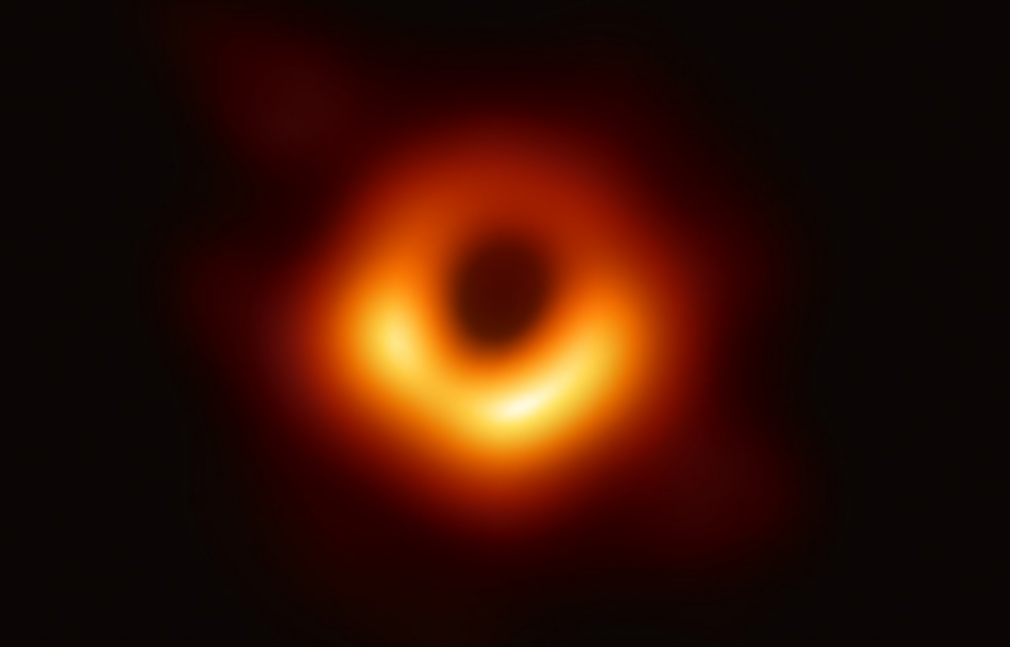
\includegraphics[scale=0.4]{img/imgRG6.1.PNG}
        \caption{Agujero negro en M87.}
    \end{center}
\end{figure}

\subsection*{Características}
\textbf{Escala:} Objetos masivos de orden de varias a millones de masas solares $3-10 M_{\odot}$. (Estelares a supermasivos)\\
\textbf{Origen:} Colapso gravitacional de una estrella, cuando se supera el límite de Tolman-Oppenheimer-Volkoft.\\
\textbf{Matemática:} Satisfacen las ecuaciones de Einstein y son buenos ejemplos de espacio-tiempos curvados donde la escala de masa hace que $GM/c^2>>1$.\\
\textbf{Características:} BH astrofísicos vienen caracterizados por su masa $M$, espin $J$ y carga $Q$.

\section{Agujero negro de Schwarzschild}
La métrica para un espacio-tiempo curvado por un objeto de masa $M$, estático y sin carga viene dado por:
\begin{equation}
    \mathrm{d}s^2=-\left(1-\dfrac{2GM}{r}\right)\mathrm{d}t^2+\left(1-\dfrac{2GM}{r}\right)^{-1}\mathrm{d}r^2+r^2(\mathrm{d}\theta^2+\sin^2 \theta\mathrm{d}\varphi)
\end{equation}

Este espacio-tiempo tiene las siguientes propiedades:\\
\textbf{Singularidad:} En $r=0$ y en $r=2GM$.\\
\textbf{Curvatura:} $R=0$ puesto que es solución a las ecuaciones de Einstein.\\
\textbf{Kretschmann scalar:} Dado por $R^{\mu\nu\rho\theta}R_{\mu\nu\rho\theta}=\dfrac{48G^2M^2}{r^6}$.\\
\textbf{Conos de luz:} ``Cerrados'' en $r=2GM$.\\
\textbf{Horizonte de eventos:} Se define como el punto de no retorno, y ocurre en el \textcolor{red}{radio de Schwarzschild}, la cual nos da una escala para considerar efectos gravitacionales
\begin{equation}
    R_{\oplus}=\dfrac{2GM_{\oplus}}{c^2}\approx 8.9mm,\quad R_{\ominus}=\dfrac{2GM_{\ominus}}{c^2}\approx 3km.
\end{equation}

Distribuciones de masa con radio del orden del radio de Schwarzschild colapsan y forman agujeros negros.

El límite de masa para formar un agujero egro astrofísico viene dado por:
\begin{equation}
    M>4M_{\odot} \rightarrow \ \text{Límite de Tolman-Oppenheimer-Volkoff}
\end{equation}

\begin{figure}[h]
    \centering
    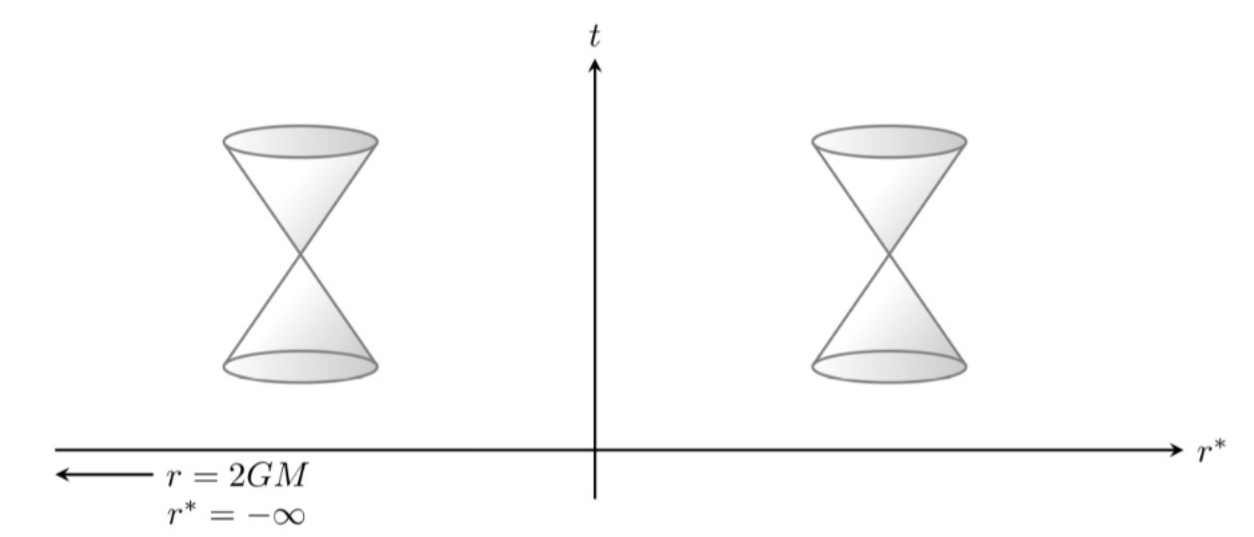
\includegraphics[scale=0.5]{img/imgRG6.2.PNG}
    \caption{Conos de luz cerrándose para un observador distante.}
\end{figure}

Los conos de luz satisfacen:
\begin{equation}
    \dv{t}{r}=\pm\left(1-\dfrac{2GM}{r}\right)^{-1};\ \dv{t}{r}\rightarrow \pm \infty
\end{equation}
sin embargo, en $r=2GM$, ningun invariante del tensor de curvatura es singular. 

(Solución: cambio de coordenadas)

Para demostrar que el espacio-tiempo de una distribución de masa $M$, estática y sin carga no es singular en $r=2GM$ usamos un cambio de coordenadas tal que, el push-forward de las funciones coordenadas $\varphi$ y $\psi$ satisfaga:
\begin{equation}
    (\psi \circ \varphi^{-1})* \pdv{}{x^{i}}\Big{|}_{\varphi(p)}=\pdv{\tilde{x}^j}{x^{i}}(\varphi(p))\pdv{}{\tilde{x}^j}\Big{|}_{\psi(p)}
\end{equation}

Para resolver el problema de los conos de luz en la métrica de Schwarzschild usamos varios cambios de coordenadas.

\subsection{Coordenadas Regge-Wheeler}

Se introduce remapeando $r=2GM$ a infinito, usando el cambio de variables
\begin{equation}
    r^*=r+2GM\ln\left(\dfrac{r}{2GM}-1\right),
\end{equation}
donde $r^*$ se conoce como la \textcolor{red}{coordenada tortuga} de $r$, donde en $r\rightarrow 2GM$, $r^* \rightarrow +\infty$. Las coordenadas modifican los conos de luz manteniendolos constantes:
\begin{figure}[h]
    \begin{center}
        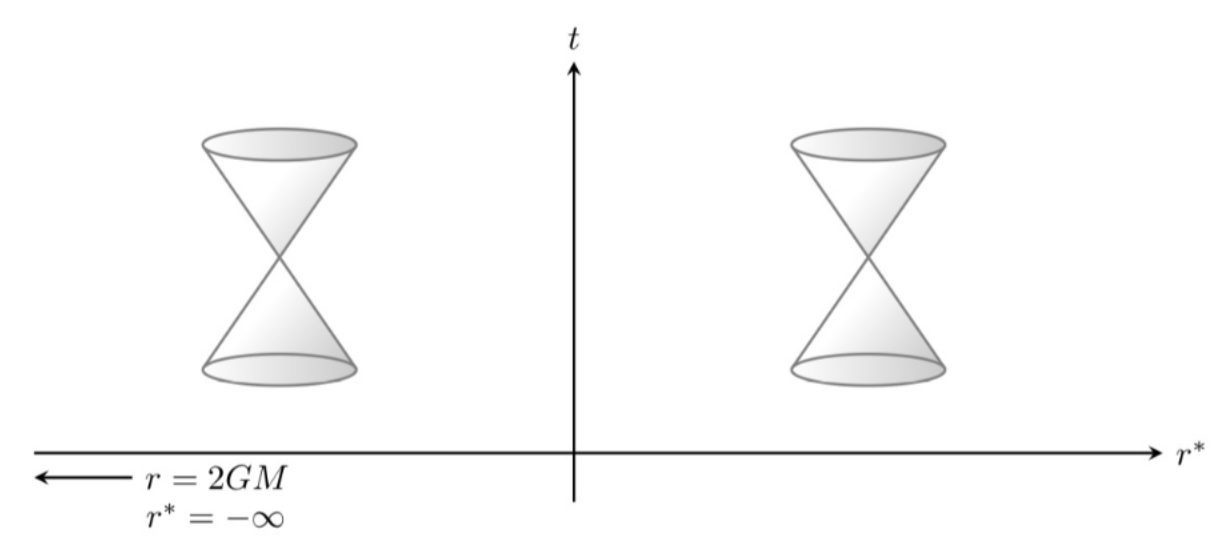
\includegraphics[scale=0.5]{img/imgRG6.3.PNG}
        \caption{Conos de luz en coordenadas tortuga.}
    \end{center}
\end{figure}

\begin{equation}
    \dv{t}{r}=\pm\left(1-\dfrac{2GM}{r}\right)^{-1},\quad \dv{t}{r^*}=\pm 1,\quad t=\pm r^*+C
\end{equation}

En estas coordenadas escribimos la métrica $\mathrm{d}s^2$ como:
\begin{equation}
    \mathrm{d}s^2=\left(1-\dfrac{2GM}{r}\right)(-\mathrm{d}t^2+\mathrm{d}r^*{}^2)+r^2\mathrm{d}\Omega
\end{equation}

Esta métrica no es singular en $r=2GM$, sin embargo estos puntos están en $r^*=\pm \infty$ para ver que ocurre en la superficie $r=2GM$ usamos otro cambio de coordenadas.

\subsection{Coordenadas de Eddington-Finkelstein}

Podemos adaptar las coordenadas para las geodésicas nulas usando el siguiente cambio de coordenadas:
\begin{equation}
    \begin{split}
        v&=t+r^*\\
        u&=t-r^*
    \end{split}
\end{equation} 

Usando este cambio de variables podemos escribir la métrica como:
\begin{equation}
    \mathrm{d}s^2=-\left(1-\dfrac{2GM}{r}\right)\mathrm{d}v^2+(\mathrm{d}v\mathrm{d}r+\mathrm{d}r\mathrm{d}v)+r^2\mathrm{d}\Omega^2
\end{equation}
vemos que $g_{vv}=0$ para $r=2GM$, sin embargo el tensor métrico \textcolor{red}{no es degenerado}.
\begin{equation}
    \det(g)=-r^4 \sin^2 \theta
\end{equation}

Notamos que de la definición de $r^*$ tenemos que:
\begin{equation}
    v=2r+4GM\ln \left| \dfrac{r}{2GM}-1 \right|+C
\end{equation}
donde esta coordenada asume que la coordenada $r^*$ es válida en ambos lados del horizonte de eventos.

En esta coordenada $r^* \in (-\infty, +\infty)$ fuera del horizonte y $r^* \in (-\infty, 0)$ dentro del horizonte y la singularidad $r=0$ está en $r^*=0$. Las geodésicas nulas $r^+$ fuera del horizonte satisfacen:

\begin{minipage}{0.5\textwidth}
    \begin{align}
        v&=2r+4GM\ln\left|\dfrac{r}{2GM}-1\right|+C \tag{$r^+$}\\
        v&=C \tag{$r^-$}
    \end{align}
\end{minipage}
\begin{minipage}{0.5\textwidth}
    \begin{center}
        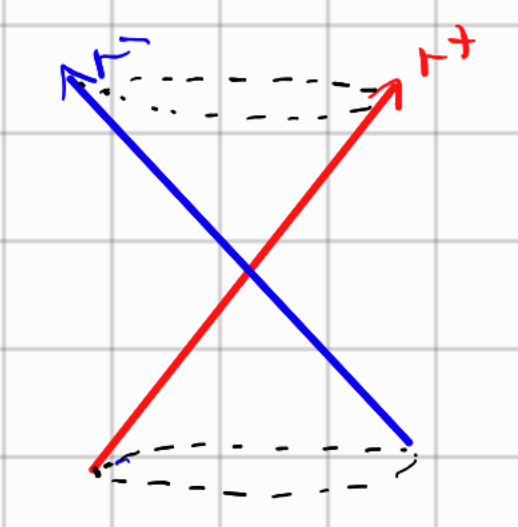
\includegraphics[scale=0.3]{img/imgRG6.4.PNG}
    \end{center}
\end{minipage}

Entonces los conos de luz en estas coordenadas son:
\begin{equation}
    \dv{v}{r}\left\{
    \begin{array}{cc}
        0 & ,r^-\\
        2\left(1-\dfrac{2GM}{r}\right)^{-1} & ,r^+
    \end{array}
    \right.
\end{equation}

\begin{figure}[h]
    \begin{center}
        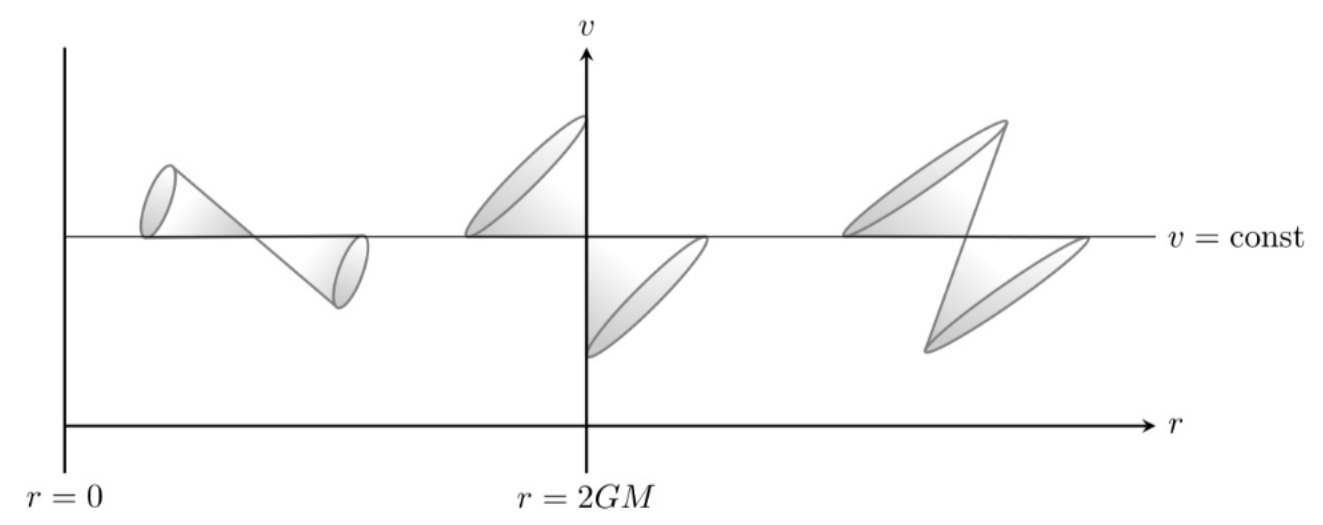
\includegraphics[scale=0.4]{img/imgRG6.5.PNG}
        \caption{Conos de luz en coordenadas Eddington-Finkelstein}
    \end{center}
\end{figure}

Nótese que:
\begin{enumerate}
    \item No existe singularidad en $r=2GM$.
    \item $\dv{v}{r}$ cambia de signo en $r<2GM$.
    \item Vemos que todas las geodésicas time-like para $r<2$ están ``atrapadas'' dentro de $r=2GM$.
\end{enumerate}

Para mostrar explícitamente que $r=2GM$ define un agujero negro usamos un \textcolor{red}{diagrama de Finkelstein} definiendo:
\begin{equation}
    v=t+r^*=t^*+r
\end{equation}
esto es $t^*=v-r$, usando la definición de $v$ tenemos que:
\begin{equation}
    t^*\left\{
    \begin{array}{cc}
        -r+C &, \text{para} \ r^-\\
        r+4GM\ln\left|1-\dfrac{2GM}{r}\right|+C &, \text{para} \ r^+
    \end{array}
    \right.
\end{equation}
\begin{figure}[h]
    \begin{center}
        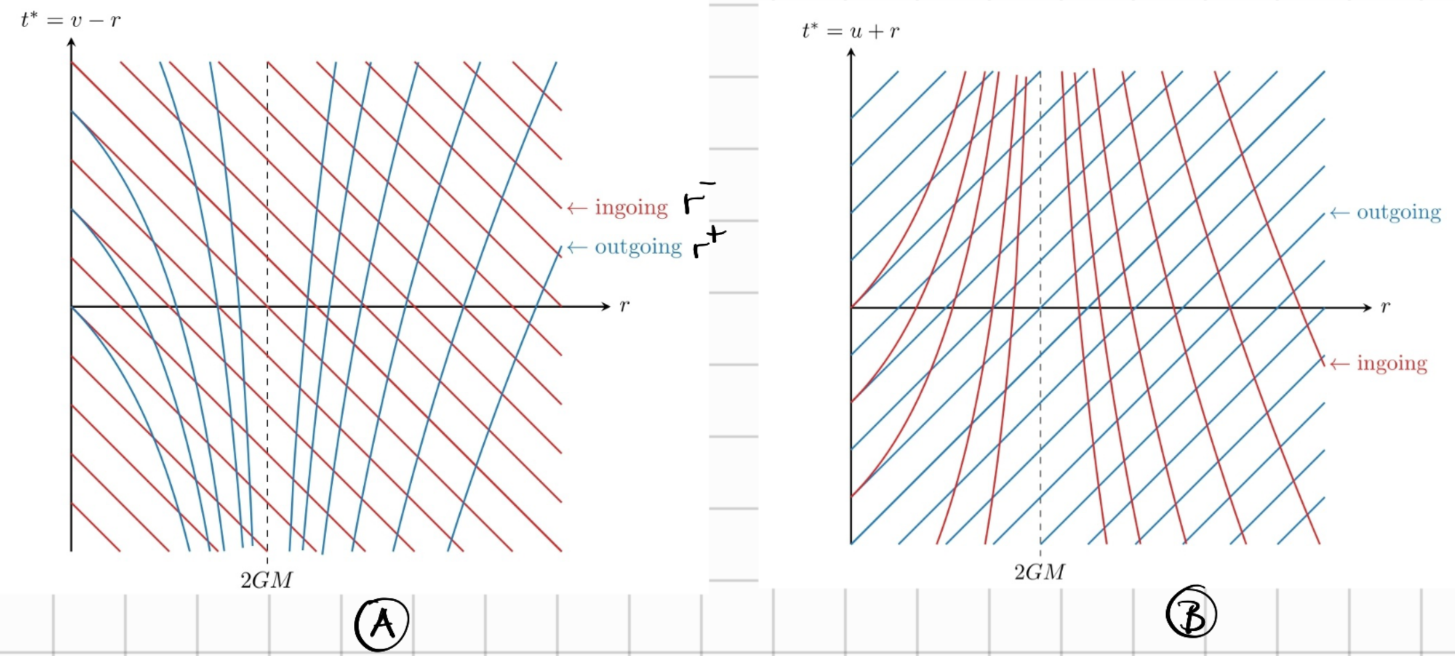
\includegraphics[scale=0.4]{img/imgRG6.6.PNG}
    \end{center}
    \caption{Diagrama de Finkelstein para $t^*=v-r$ (A), y para $t^*=v+r$ (B).}
\end{figure}
Esta elección de coordenadas $t^*=v-r$ puede ser dada también para $t^*=v+r$, donde este caso corresponde a la inversiones temporal $t\rightarrow -t$. Donde al escoger
\begin{equation}
    u=t-r^*
\end{equation}
la métrica nos queda:
\begin{equation}
    \mathrm{d}s^2=-\left(1-\dfrac{2GM}{r}\right)\mathrm{d}u^2-\mathrm{d}u\mathrm{d}r+r^2\mathrm{d}\Omega^2
\end{equation}

En estas coordenadas vemos que el pasado de los conos de luz consiguen ``salir'' del horizonte de eventos entonces se dice que estas coordenadas describen en \textcolor{red}{agujero blanco}, puesto que se trata de un agujero negro con ``tiempo invertido''.\footnote{Esto viene del hecho de que las ecuaciones de Einstein son invariantes bajo transformaciones de inversión de tiempo $t\rightarrow -t$.}

A pesar de que definamos estas coordenadas, existen los siguientes problemas:
\begin{enumerate}
    \item $v(r)$ diverge para $r\rightarrow 2GM$ con $r=\sqrt{2GM\tau}$
    \begin{equation}
        v(r)=\int \left(1-\dfrac{2GM}{r}\right)^{-1}\mathrm{d}\tau
    \end{equation}
    \item La región con $v$ finito dentro del agujero negro es diferente de la región $u$ finito para $r<2GM$.
    \item El horizonte del agujero negro para $v$ finito es distinto del caso $u$ finito a pesar de que describen el mismo objeto en la manifold.
\end{enumerate}

Antes de mostrar como resolver estos problemas introduciremos las coordenadas de Rindler.

\subsection{Coordenadas de Rindler}

Para la métrica de Schwarzschild podemos aproximar la coordenada $r$ como:
\begin{equation}
    \begin{split}
        r=2GM+\eta,\quad \text{con} \ 0\leq \eta << 2GM\\
        g_{tt}=1-\dfrac{2GM}{r}\approx \dfrac{\eta}{2GM}+\mathcal{O}(\eta^2) \ \text{para} \ \eta << 2GM
    \end{split}
\end{equation}
en este límite 
\begin{equation}
    \mathrm{d}s^2=\underbrace{-\dfrac{\eta}{2GM}\mathrm{d}t^2+\dfrac{2GM}{\eta}\mathrm{d}\eta^2}_{\textcolor{red}{\text{espacio-tiempo de Rindler}}}+\underbrace{(2GM)^2\mathrm{d}\Omega^2}_{\textcolor{red}{s^2}}
\end{equation}

Cambiando variables $\rho^2=8\pi GM \eta$, el espacio-tiempo de Rindler nos queda:
\begin{equation}
    \mathrm{d}s^2=-\left(\dfrac{\rho}{4GM}\right)\mathrm{d}t^2+\mathrm{d}\rho^2
\end{equation}

En este espacio-tiempo un observador con $\rho=cte$ está acelerado $a^{\mu}=u^{\nu}\nabla_{\nu}u^{\mu}\neq 0$ donde $u^{\mu}$ es la cuadri-velocidad $\displaystyle\dv{x^{\mu}}{T}$, vemos que al introducir las coordenadas:
\begin{equation}
    T=\rho \sinh\left(\dfrac{t}{4GM}\right),\quad X=\rho \cosh\left(\dfrac{t}{4GM}\right)
\end{equation}
la métrica de Rindler satisface:
\begin{equation}
    \mathrm{d}s^2=-\mathrm{d}T^2+\mathrm{d}X^2,\quad X\in (0, \infty), \quad -X< T < X
\end{equation}
reduciéndose a una métrica de Minkowski
\begin{figure}[h]
    \begin{center}
        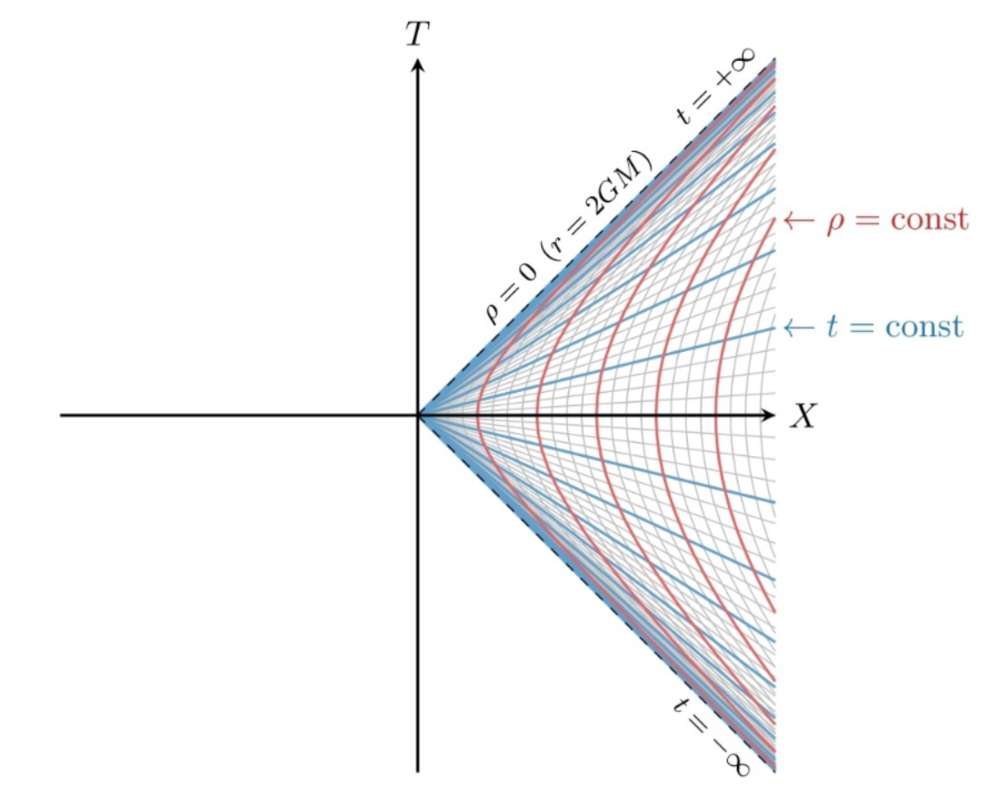
\includegraphics[scale=0.4]{img/imgRG6.7.PNG}
        \caption{Espacio-tiempo cubierto por la métrica de Rindler.}
    \end{center}
\end{figure}

Dado que para $t\rightarrow \pm \infty$ y $\rho \rightarrow 0$ vemos que el horizonte de eventos es una \textcolor{red}{superficie nula}.

\textcolor{red}{Comentario:} Vemos que en general, como ocurre con observadores acelerados no todos los cambios de variable cubren todo el espacio-tiempo. Para el caso del espacio-tiempo de Schwarzschild las coordenadas de Kruskal resuelven este problema.

\section{Campos escalares en la geometría de Schwarzschild}

La acción de un campo escalar libre sin masa viene dada por:
\begin{equation}
    S[\phi]=\int \mathrm{d}^4 x \sqrt{-g} g^{\alpha\beta}\partial_{\alpha} \phi \partial_{\beta} \phi
\end{equation}
usando las coordenadas tortuga escribimos
\begin{equation}
    S[\phi]=\int \mathrm{d}t\mathrm{d}r^* \mathrm{d}\Omega \left[-(r\partial_t \phi)^2+(r\partial_{r^*} \phi)^2-f(r)\phi \Box_{s^2}\phi \right]
\end{equation}
donde $\displaystyle f(r)=1-\dfrac{2GM}{r}$, $\mathrm{d}\Omega=\sin \theta \mathrm{d}\theta \mathrm{d}\varphi$ y $\Box_{s^2}$ es el laplaciano en la 2-esfera.

Usando la expansión en armónicos esféricos para el campo escalar $\phi$:
\begin{equation}
    \phi=\dfrac{1}{r}\sum_{l, m} \psi_{lm}(t, r^*) Y_{lm}(\theta, \varphi)
\end{equation}
usando las identidades:
\begin{align}
    \Box_{s^2}Y_{l, m}&=-l(l+1)Y_{lm} &(\text{Armónicos esféricos})\\
    r\partial_{r^*}(\psi_{lm}/r)&=\partial_{r^*}\psi_{lm}-r^{-1}f(r)\psi_{lm} &(\text{Regla de la cadena})
\end{align}

Encontramos la ecuación de movimiento:
\begin{equation}
    (\partial^2_t-\partial^2_{r^*})\psi_{lm}+V_e(r^*)\psi_{lm}=0
\end{equation}
donde $V_e$ es el potencial para el campo escalar $\phi$:
\begin{equation}
    V_e(r^*)=\left(1-\dfrac{2M}{r}\right)\left(\dfrac{l(l+1)}{r^2}+\dfrac{2m}{r^3}\right)
\end{equation}

Notamos que para $\phi=e^{-i\omega t}\psi(r^*)$, obtenemos:
\begin{equation}
    -\partial^2_{r^*}\psi_{lm}+V_e(r^*)\psi_{lm}=\omega^2 \psi_{lm}
\end{equation}
que nos da una ecuación de tipo Schrödinger. Esta ecuación junto con su equivalente para vectores y tensores se conoce como las ecuaciones de Regge-Wheeler-Zerilli.
\begin{figure}[h]
    \centering
    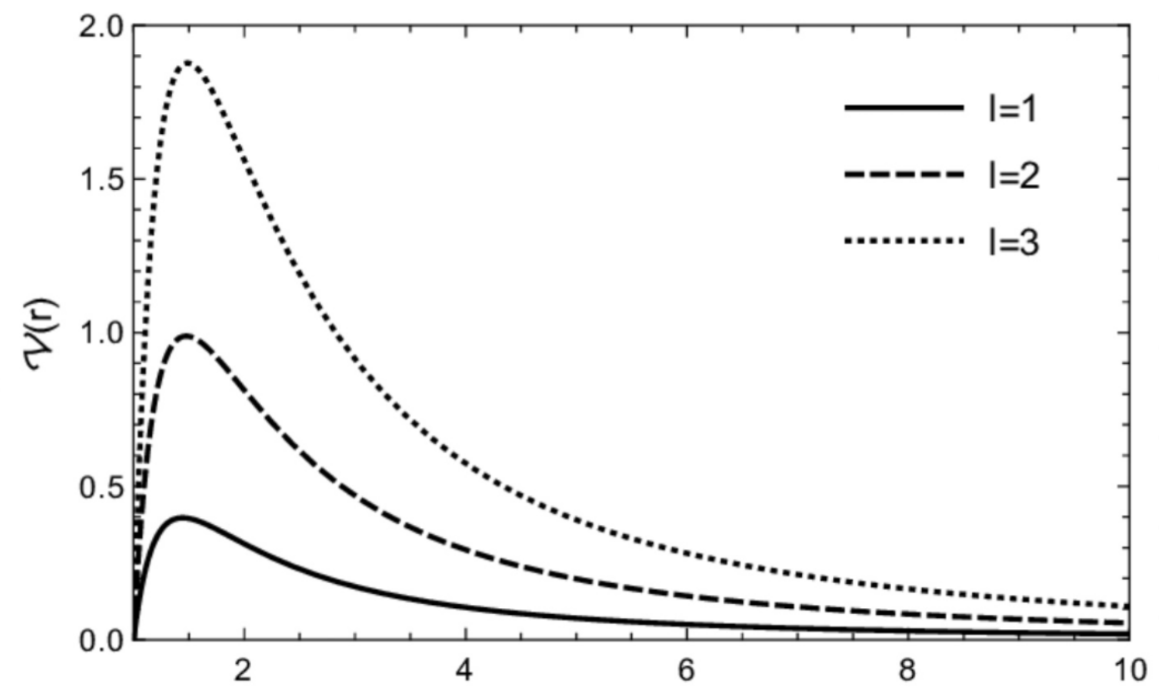
\includegraphics[scale=0.5]{img/imgRG6.8.PNG}
    \caption{Potencial de Regge-Wheeler para un campo escalar en la métrica de Schwarzschild.}
\end{figure}

\subsection{Coordenadas de Kruskal}

La idea en estas coordenadas es usar las coordenadas nulas $v, u$ para la métrica de Schwarzschild
\begin{equation}
    \begin{split}
        \mathrm{d}s^2&=\left(1-\dfrac{2GM}{r}\right)(-\mathrm{d}t^2+\mathrm{d}r^*{}^2)+r^2\mathrm{d}\Omega^2\\
        &=-\left(1-\dfrac{2GM}{r}\right)\mathrm{d}u\mathrm{d}v+r^2\mathrm{d}\Omega^2
    \end{split}
\end{equation}
donde $u=t-r^*$ y $v=t+r^*$ y $r^2$ es una función de $u-v$. Se define el sistema de coordenadas de Kruskal usando los siguientes cambios de variable
\begin{equation}
    u=-\exp\left[\dfrac{-u}{4GM}\right],\quad v=\exp\left[\dfrac{v}{4GM}\right]
\end{equation}

vemos que, el exterior del agujero negro corresponde a $u<0$ y $v>0$ del horizonte:
\begin{equation}
    \begin{split}
        uv&=\exp\left[\dfrac{r^*}{2GM}\right]\\
        u/v&=-\exp\left[-\dfrac{t}{2GM}\right]
    \end{split}
\end{equation}

Por lo tanto la métrica:
\begin{equation}
    \mathrm{d}s^2=-\dfrac{32(GM)^3}{r}e^{-r/2GM}\mathrm{d}u\mathrm{d}v+r^2\mathrm{d}\Omega^2
\end{equation}

\textcolor{red}{Notamos:}
\begin{enumerate}
    \item La métrica de Schwarzschild es cubierta por la región con $u<0$ y $v>0$.
    \item Las coordenadas $u$ y $v$ son coordenadas nulas para $\partial_u$ y $\partial_v$.
    \item Se puede llevar a un sistema de coordenadas donde una coordenada es de tipo time-like y la otra space-like:
    \begin{align}
        T&=\dfrac{1}{2}(v+u)=\left(\dfrac{r}{2GM}-1\right)^{1/2}e^{r/4GM}\sinh\left(\dfrac{t}{4GM}\right)\\
        X&=\dfrac{1}{2}(v-u)=\left(\dfrac{r}{2GM}-1\right)^{1/2}e^{r/4GM}\cosh\left(\dfrac{t}{4GM}\right)
    \end{align}
    usando esta forma nos queda:
    \begin{equation}
        \mathrm{d}s^2=\dfrac{32(GM)^3}{r}e^{-r/2GM}(-\mathrm{d}T^2+\mathrm{d}X^2)+r^2\mathrm{d}\Omega^2
    \end{equation}
    con $r$ siendo una función implícita dada por la condición:
    \begin{equation}
        T^2-X^2=\left(1-\dfrac{r}{2GM}\right)\exp\left[\dfrac{r}{2GM}\right]
    \end{equation}
    \item Las geodésicas nulas satisfacen:
    \begin{equation}
        T=\pm X+C
    \end{equation}
    \item El horizonte de eventos($r=2GM$) se encuentra en la hipersuperficie:
    \begin{equation}
        T=\pm X
    \end{equation}
    \item El horizonte de eventos es una superficie \textcolor{red}{nula} en estas coordenadas.
    \item El espacio-tiempo es similar al de Rindler puesto que:
    \begin{equation}
        \dfrac{T}{X}=\tanh\left(\dfrac{t}{4GM}\right)
    \end{equation}
    para $t\rightarrow \pm \infty$, $r \rightarrow 2GM$.
\end{enumerate}

\subsection{Diagrama de Kruskal}

\begin{figure}[h]
    \centering
    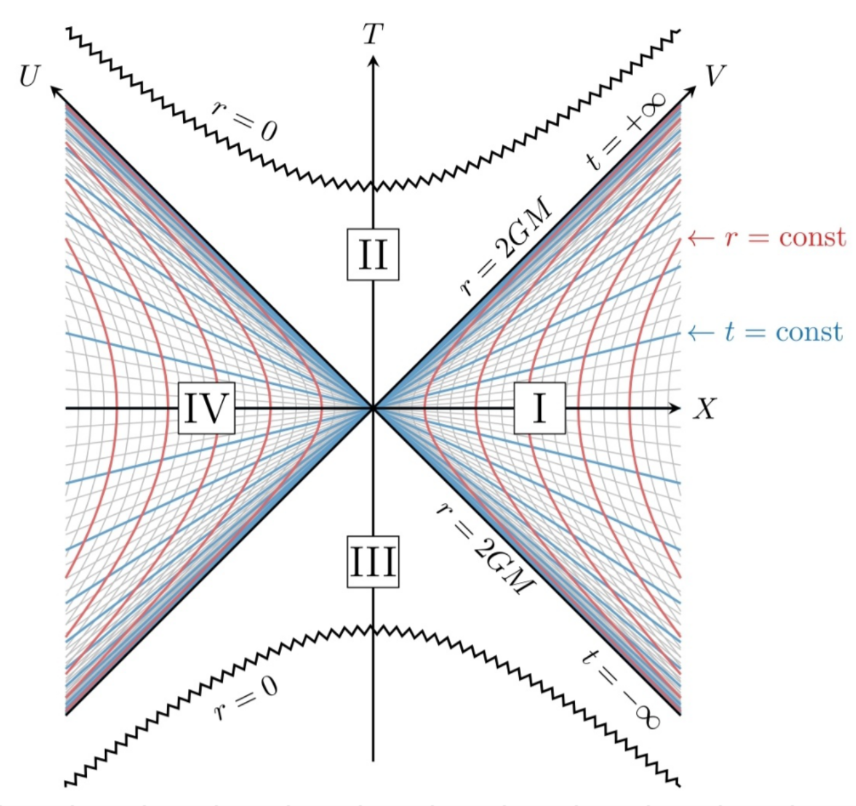
\includegraphics[scale=0.5]{img/imgRG6.9.PNG}
    \caption{Diagrama de Kruskal para el agujero negro de Schwarzschild.}
\end{figure}

En este diagrama tenemos:
\begin{enumerate}
    \item $r=2GM$ es decir $T=\pm X$, entonces $uv=0$.
    \item La superficie $T=X$ es el horizonte del \textcolor{red}{agujero negro}.
    \item La superficie $T=-X$ es el horizonte del \textcolor{red}{agujero blanco}.
    \item La región I es el espacio-tiempo fuera del agujero negro con $T \in [2GM, +\infty)$.
    \item La región II es el espacio-tiempo dentro del agujero negro(Contiene la singularidad $r=0$) \textcolor{red}{(está siempre en el futuro).}
    \item La región III es el espacio-tiempo dentro del agujero blanco(Contiene la singularidad $r=0$) \textcolor{red}{(está siempre en el pasado).}
    \item La región IV es otra copia del espacio-tiempo fuera del agujero negro \textcolor{red}{causalmente desconectada} de la región I. Donde tenemos:
    \begin{align}
        u&=+\exp\left[\dfrac{u}{4GM}\right]\\
        v&=-\exp\left[-\dfrac{v}{4GM}\right]
    \end{align}
    esta región tiene $u>0$ y $v<0$.
    \item El \textcolor{red}{vector de Killing} cambia de signo al cruzar el horizonte 
    \begin{equation}
        K=\pdv{}{t}=\dfrac{1}{4GM}\left(v\pdv{}{v}-u\pdv{}{u}\right)
    \end{equation}
    la norma en las coordenadas de Kruskal viene dada por:
    \begin{equation}
        g_{\mu\nu}K^{\mu}K^{\nu}=-\left(1-\dfrac{2GM}{r}\right)
    \end{equation}
    para $r>2GM$, $K^2<0$(time-like) \textcolor{red}{(espacio-tiempo estacionario).}\\
    para $r<2GM$, $K^2>0$(space-like) \textcolor{red}{(espacio-tiempo no estacionario).}
    \item Existe un \textcolor{red}{agujero de gusano} que ``conecta'' la región I y IV pero con distancias space-like(no se puede cruzar). Esto también se llama \textcolor{red}{puente de Einstein-Rosen.}
\end{enumerate}

\section{Diagramas de Penrose}

Son representaciones compactas de espacios-tiempo.

\subsection{Minkowski(2D)}
El espacio-tiempo de Minkowski se puede representar de forma conformal, introduciendo las coordenadas nulas:
\begin{equation}
    u=t-x,\quad v=t+x,\quad x \in (-\infty, +\infty)
\end{equation}

La métrica se reduce a:
\begin{equation}
    \mathrm{d}s^2=-\mathrm{d}u\mathrm{d}v\quad u,v \in (-\infty, +\infty)
\end{equation}
para mapear esta métrica a un espacio finito usamos:
\begin{equation}
    \begin{split}
        u&=\tan \bar{u}\quad \bar{u}, \bar{v} \in (-\pi/2, \pi/2)\\
        v&=\tan \bar{v} 
    \end{split}
\end{equation}
en estas coordenadas tenemos:
\begin{equation}
    \mathrm{d}s^2=-\dfrac{1}{\cos^2 \bar{u} \cos^2 \bar{v}}\mathrm{d}\bar{u}\mathrm{d}\bar{v}
\end{equation}
y notamos que los conos de luz se mantienen y $\cos^2 \bar{u} \cos^2 \bar{v}$ es un factor \textcolor{red}{conformal} para Minkowski tenemos:
\begin{figure}[h]
    \centering
    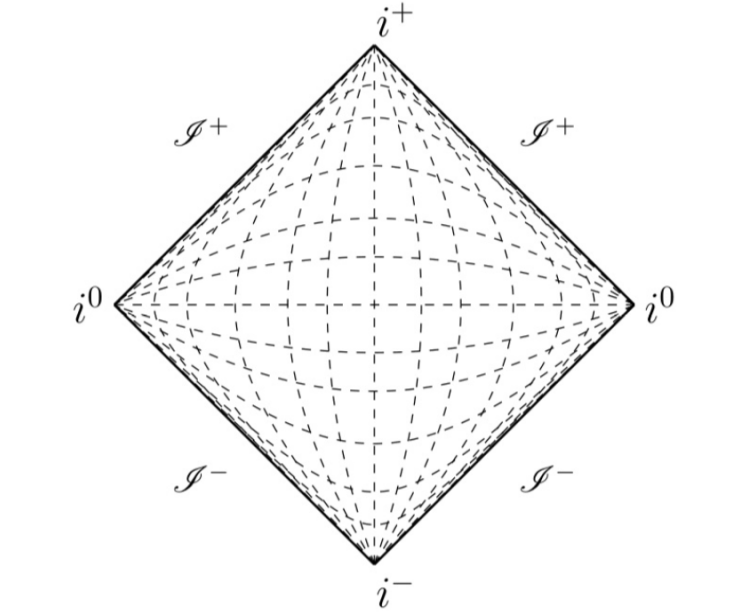
\includegraphics[scale=0.4]{img/imgRG6.10.PNG}
    \caption{Diagrama de Penrose para el espacio-tiempo de Minkowski en 2D.}
\end{figure}

En este diagrama tenemos:
\begin{itemize}
    \item \textcolor{blue}{$i^{\pm}$:} Geodésicas tipo time-like que comienzan en $i^-$ con $\bar{u}, \bar{v}=(-\pi/2, -\pi/2)$ y terminan en $\bar{u}, \bar{v}=(\pi/2, \pi/2)$. Estos puntos son el infinito de las geodésicas tipo time-like \textcolor{red}{$i^-$ (pasado)} y \textcolor{red}{$i^+$ (futuro).}
    \item \textcolor{blue}{$i^{0}$:} Todas las geodésicas tipo space-like comienzan y terminan en este punto y son el infinito, $i^{0}$ puede ser $\bar{u}, \bar{v}=(-\pi/2, \pi/2)$ para $+\infty$ y $\bar{u}, \bar{v}=(\pi/2, -\pi/2)$ para $-\infty$.
    \item \textcolor{blue}{$\mathcal{J}^{\pm}$:} Todas las geodésicas \textcolor{red}{nulas} comienzan con $\mathcal{J}^-$ ($\bar{u}, \bar{v}=-\pi/2, -\pi/2$) y terminan con $\mathcal{J}^+$ ($\bar{u}, \bar{v}=\pi/2, \pi/2$). $\mathcal{J}^-$ es el \textcolor{red}{pasado} de las geodésicas nulas y $\mathcal{J}^+$ es el futuro de las geodésicas nulas.
\end{itemize}

\subsection{Minkowski en 4D}

En $3+1$ tenemos:
\begin{equation}
    \mathrm{d}s^2=-\mathrm{d}t^2+\mathrm{d}r^2+r^2\mathrm{d}\Omega^2
\end{equation}
en coordenadas nulas tenemos:
\begin{equation}
    u=t-r\qquad v=t+r
\end{equation}
la métrica se escribe en estas coordenadas como:
\begin{equation}
    \mathrm{d}s^2=-\mathrm{d}u\mathrm{d}v+\dfrac{1}{4}(u-v)\mathrm{d}\Omega^2
\end{equation}
el cual al usar el mismo mapeo para $1+1$ dimensiones:
\begin{equation}
    \mathrm{d}s^2=\underbrace{\dfrac{1}{4\cos^2 \bar{u} \cos^2 \bar{v}}}_{\text{factor conformal}} \underbrace{(-4\mathrm{d}\bar{u}\mathrm{d}\bar{v}+\sin^2(\bar{u}-\bar{v})\mathrm{d}\Omega^2)}_{\mathrm{d}s'{}^2}
\end{equation}
analizamos $\mathrm{d}s'{}^2$ al ser equivalente a $\mathrm{d}s^2=0$ en este caso como $r>0$ (en el caso anterior $X$ no tenia por que serlo)
\begin{equation}
    v-u=2r \ \rightarrow \ v>0 \ \text{tal que} \ r>0
\end{equation}

Esto limita los valores de $\bar{u}$ y $\bar{v}$
\begin{equation}
    -\dfrac{\pi}{2}\leq \bar{u} \leq \bar{v} \leq \dfrac{\pi}{2}
\end{equation}
\begin{figure}[h]
    \begin{minipage}{0.6\textwidth}
        \centering
            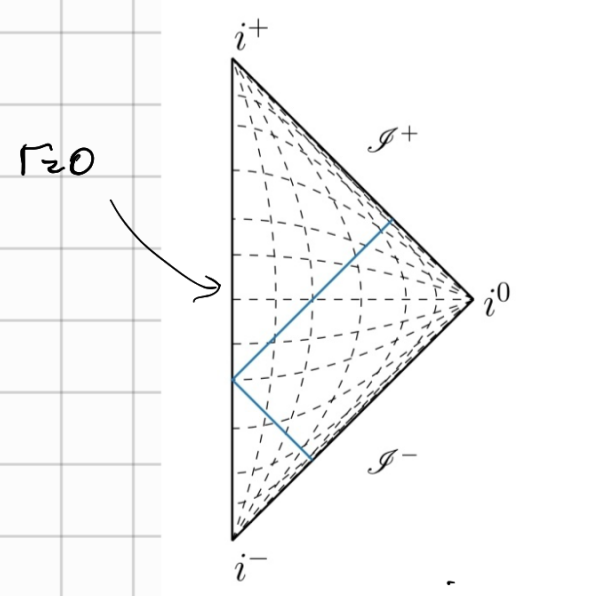
\includegraphics[scale=0.5]{img/imgRG6.11.PNG}
            \caption{Diagrama de Penrose para Minkowski en $3+1$.}
    \end{minipage}
    \begin{minipage}{0.4\textwidth}
        En $r=0$, los rayos de luz son reflejados hacia el futuro de las geodésicas nulas $\mathcal{J}^+$.
        \\
        Esto pasa por constricción (es decir $r\geq 0$).
    \end{minipage}
\end{figure}

\subsubsection{Schwarzschild}

Para este caso usemos las coordenadas de Kruskal
\begin{equation}
    \mathrm{d}s^2=-\dfrac{32(GM)^3}{r}e^{-r/2GM}\mathrm{d}u\mathrm{d}v+r^2\mathrm{d}\Omega^2
\end{equation}

Definamos la transformación
\begin{equation}
    u=\tan \bar{u},\quad v=\tan \bar{v},\quad \bar{u}, \bar{v} \in (-\pi/2, \pi/2)
\end{equation}
la métrica se transforma en:
\begin{equation}
    \mathrm{d}s^2 = \dfrac{1}{\cos^2 \bar{u} \cos^2 \bar{v}} \left[-\dfrac{32(GM)^3}{r}e^{-r/2GM}\mathrm{d}\bar{u}\mathrm{d}\bar{v}+r^2\cos^2 \bar{u}\cos^2 \bar{v}\mathrm{d}\Omega^2\right]
\end{equation}
la singularidad en $r=0$, $uv=1$ está dada en:
\begin{equation}
    \begin{split}
        \tan \bar{u} \tan \bar{v} &=1 \\
        \cos(\bar{u}+\bar{v})&=0,\quad \bar{u}+\bar{v}=\pm \dfrac{\pi}{2}
    \end{split}
\end{equation}
\begin{figure}[h]
    \centering
    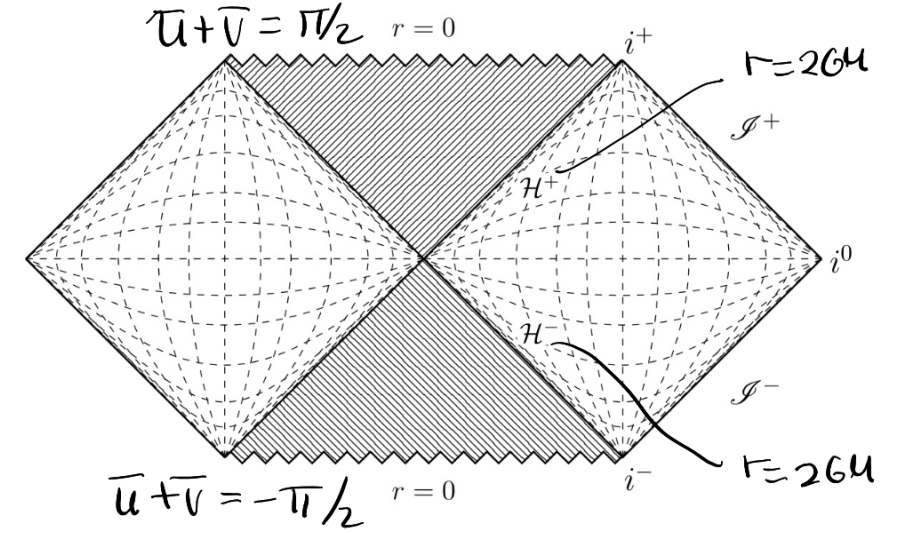
\includegraphics[scale=0.5]{img/imgRG6.12.PNG}
    \caption{Diagrama de Penrose para el agujero negro de Schwarzschild.}
\end{figure}

\section{Agujeros negros cargados}

Esta solución de agujero negro viene dada por la acción:
\begin{equation}
    S= \int \mathrm{d}^4 x \sqrt{-g}\left(\dfrac{1}{16\pi G}R-\dfrac{1}{4}F_{\mu\nu}F^{\mu\nu}\right)
\end{equation}
donde $F_{\mu\nu}=\nabla_{\mu} A_{\nu}-\nabla_{\nu}A_{\mu}$ vemos que:
\begin{equation}
    \begin{split}
        \delta S_{A_{\mu}} \ &\rightarrow \ \nabla_{\mu} F^{\mu\nu}=0\\
        \delta S_{g_{\mu\nu}} \ &\rightarrow \ R_{\mu\nu}-\dfrac{1}{2}g_{\mu\nu}R=8\pi G T_{\mu\nu}^{(A)} 
    \end{split}
\end{equation}
donde 
\begin{equation}
    T^{(A)}_{\mu\nu}=F^{\rho}_{\mu} F_{\nu\rho}-\dfrac{1}{4}F_{\alpha\beta}F^{\alpha\beta}g_{\mu\nu}
\end{equation}
es el tensor de energía-momento para $A^{\mu}$.

Si escogemos 
\begin{equation}
    A=-\dfrac{Q_e}{4\pi r}\mathrm{d}t-\dfrac{Q_m}{4\pi}\cos \theta \mathrm{d}\phi
\end{equation}
donde $Q_e$ y $Q_m$ son las cargas eléctricas y magnéticas respectivamente. Encontramos una solución al sistema de ecuaciones $\delta S_A=0$, $\delta S_g=0$ de la forma:
\begin{equation}
    \mathrm{d}s^2=-\Delta(r)\mathrm{d}t^2+\Delta^{-1}(r)\mathrm{d}r^2+r^2\mathrm{d}\Omega^2
\end{equation}
donde $\Delta(r)$ viene dada por:
\begin{equation}
    \Delta(r)=1-\dfrac{2GM}{r}+\dfrac{Q^2}{r^2},\quad Q^2=\dfrac{G}{2\pi}(Q^2_e+Q^2_m)
\end{equation}
definiendo 
\begin{equation}
    r^{\pm}=GM\pm (G^2M^2-Q^2)^{1/2}
\end{equation}
entonces tendremos
\begin{equation}
    \Delta(r)=\dfrac{1}{r^2}(r-r^+)(r-r^-)
\end{equation}

Notamos que existen \textcolor{red}{dos horizontes} $r^+$ y $r^-$, dependiendo de los valores de carga $Q$ tenemos:
\begin{itemize}
    \item \textcolor{blue}{$Q=0$:} $r^-=0$, $r^+=2GM$ el horizonte de eventos coincide con la singularidad. El horizonte $r^+$ corresponde con el horizonte de Schwarzschild.
    \item \textcolor{blue}{$|Q|>GM$:} No existe horizonte de eventos. La singularidad $r=0$ se llama \textcolor{red}{singularidad desnuda}. Estas singularidades no son físicas. La falta de singularidades de este tipo se llama \textcolor{red}{principio de censura cósmica} (en agujeros negros que rotan esta condición lleva a un límite en el momento angular del agujero negro).
    \begin{figure}[h]
        \centering
        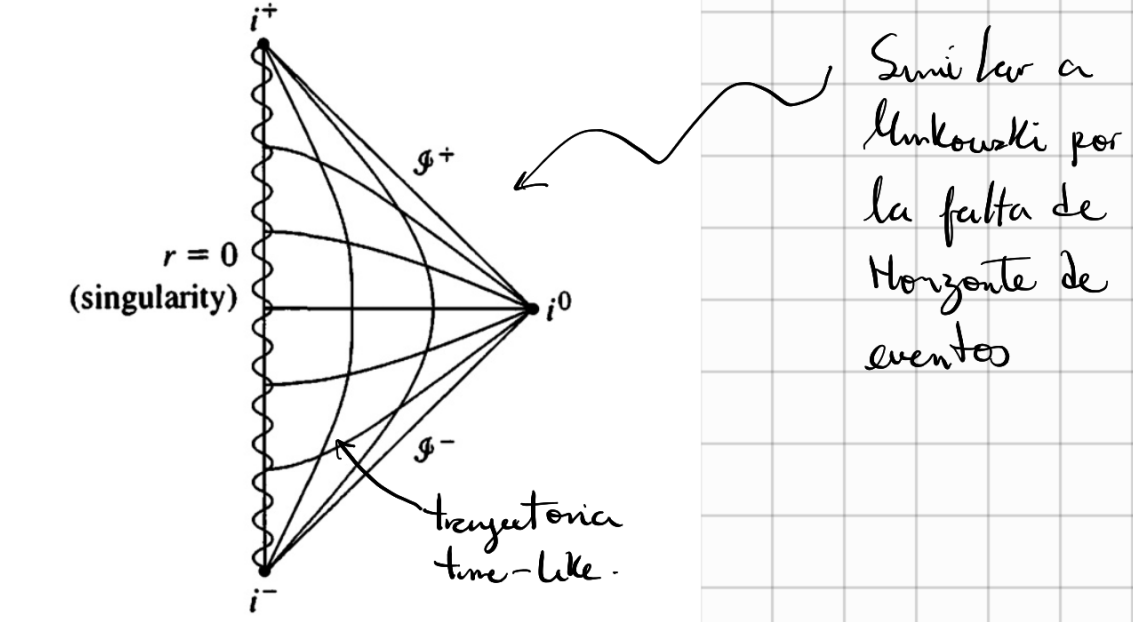
\includegraphics[scale=0.4]{img/imgRG6.13.PNG}
        \caption{Diagrama de Penrose para $|Q|>GM$.}
    \end{figure}
    \item \textcolor{blue}{$|Q|<GM$:} En este caso tenemos dos horizontes $r^+$ y $r^-$, siendo ambas superficies nulas. La singularidad pasa a ser time-like, por lo tanto es posible evitarla.
\end{itemize}
\begin{figure}[h]
    \centering
    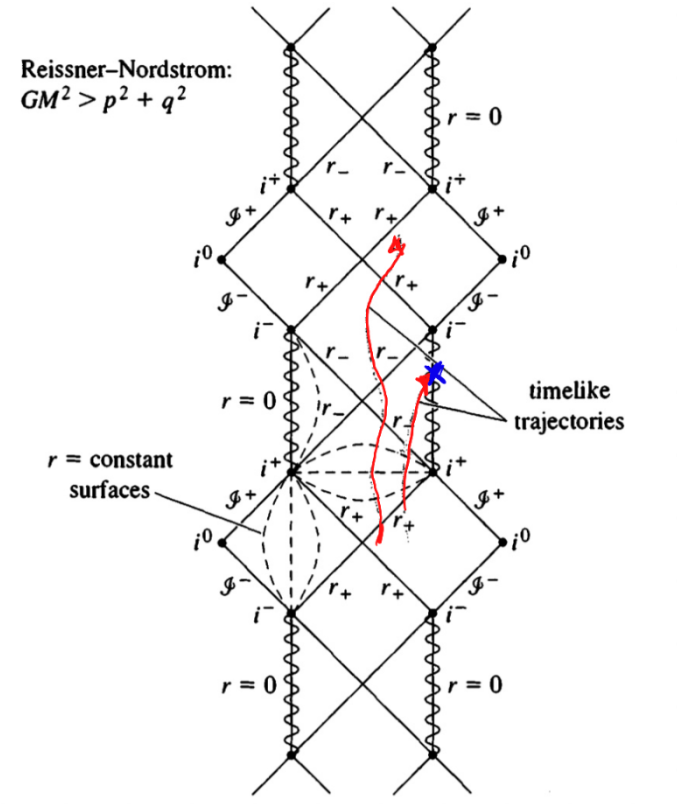
\includegraphics[scale=0.55]{img/imgRG6.14.PNG}
    \caption{Diagrama conformal para un agujero negro cargado.}
\end{figure}

\textcolor{red}{Nótese que:}

Para $r>0$, $r$ es space-like y en $r^-< r <r^+$ cambia a time-like por lo que $r\rightarrow r^-$. Luego en $r<r_-$ es de nuevo space-like y por lo tanto es posible evitar la singularidad.

\textcolor{blue}{$|Q|=GM$:} Este caso se conoce como agujero negro extremal, la métrica se traduce en:
\begin{equation}
    \mathrm{d}s^2=-\left(1-\dfrac{GM}{r}\right)^2 \mathrm{d}t^2+\left(1-\dfrac{GM}{r}\right)^{-2}\mathrm{d}r^2+r^2\mathrm{d}\Omega^2
\end{equation}
para $r=GM+\eta$ (cerca del horizonte) con $\eta<< GM$ es posible derivar:
\begin{equation}
    \mathrm{d}s^2=\underbrace{\dfrac{-\eta}{(GM)^2}\mathrm{d}t^2+\dfrac{(GM)^2}{\eta^2}\mathrm{d}\eta^2}_{\textcolor{red}{AdS_2}}+\underbrace{(GM)^2\mathrm{d}\Omega^2}_{\textcolor{red}{s^2}}
\end{equation}

Esta métrica se conoce como métrica de Robinson-Berlotti $AdS_2 \ times S^2$ y tiene geometría \textcolor{red}{anti-DeSitter}.

Para este agujero negro existen infinitas regiones extremas.
\begin{figure}[h]
    \centering
    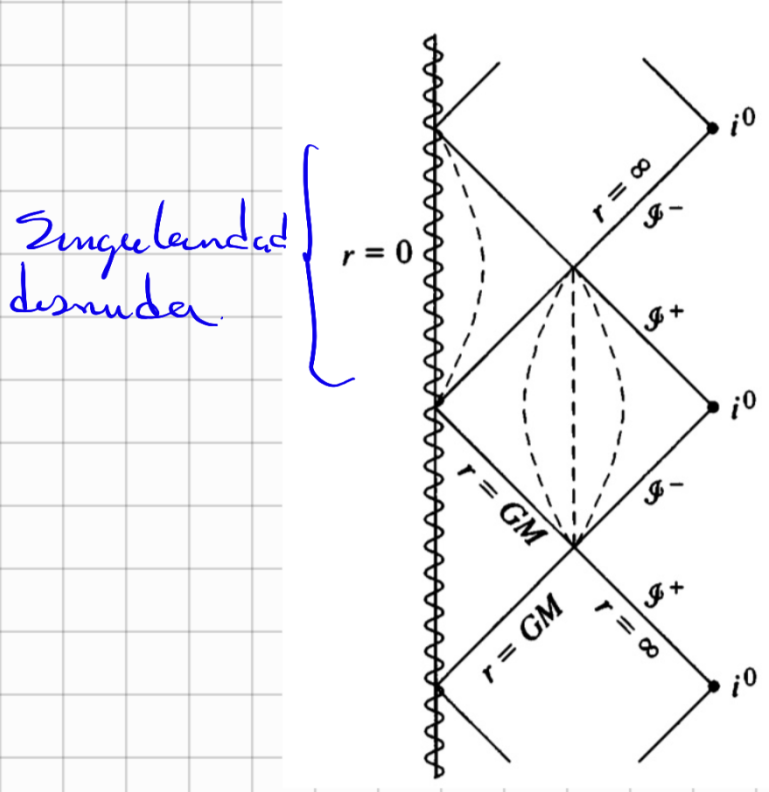
\includegraphics[scale=0.4]{img/imgRG6.15.PNG}
    \caption{Diagrama conformal para el agujero negro cargado extremal.}
\end{figure}

\section{Agujeros negros rotantes}

El agujero negro de Kerr viene dado por la métrica:
\begin{equation}
    \begin{split}
        \mathrm{d}s^2&=-\left(1-\dfrac{2GMr}{\rho^2}\right)\mathrm{d}t^2-\dfrac{2GMar\sin^2 \theta}{\rho^2}(\mathrm{d}t\mathrm{d}\phi+\mathrm{d}\phi\mathrm{d}t)+\dfrac{\rho^2}{\Delta}\mathrm{d}r^2\\
        &+\rho^2 \mathrm{d}\theta^2+\dfrac{\sin^2 \theta}{\rho^2}\left[(r^2+a^2)^2-a^2\Delta \sin^2 \theta\right]\mathrm{d}\phi^2
    \end{split}
\end{equation}
donde 
\begin{align}
    \Delta(r)&=r^2-2GMr+a^2\\
    \rho^2(r, \theta)&=r^2+a^2\cos^2 \theta
\end{align}

Donde $a$ es el \textcolor{red}{momento angular} por unidad de masa $M$. Donde $M$ (la masa del agujero negro) es la \textcolor{blue}{Masa de Komar} y $J$ el \textcolor{blue}{momento angular de Komar} definidos como 
\begin{equation}
    M_K=\dfrac{1}{4\pi G}\int_{\partial \Sigma}\mathrm{d}^2 x \sqrt{g^{(2)}} \eta_{\mu} \sigma_{\nu} \nabla^{\mu}K^{\nu}
\end{equation}
donde $g^{(2)}$ es la métrica de la 2-esfera en infinito $K^{\mu}$ es el vector de Killing, $\eta_{\mu}$ y $\sigma_{\mu}$ son vectores normalizados a 1.
\begin{equation}
    \eta_{\mu}\eta^{\mu}=-1,\quad \sigma^{\mu}\sigma_{\mu}=+1
\end{equation}

El momento angular está definido como:
\begin{equation}
    J_{Komar}=-\dfrac{1}{8\pi G}\int_{\partial \Sigma} \mathrm{d}^2 x \sqrt{g^{(2)}} \eta_{\mu} \sigma_{\nu} \nabla^{\mu} K^{\nu}_{(rot)}
\end{equation}

Las coordenadas $(t, r, \theta, \phi)$ se conocen como \textcolor{blue}{coordenadas Boyer-Lindquist}. Como en el caso del agujero negro cargado tenemos:
\begin{enumerate}
    \item \textcolor{blue}{$a> GM$:} Singularidad desnuda.
    \item \textcolor{blue}{$a = GM$:} Agujero negro extremal.
    \item \textcolor{blue}{$a < GM$:} Agujero negro en rotación, en este caso existen dos horizontes de eventos dados por:
    \begin{equation}
        r^{\pm}=GM\pm \sqrt{G^2M^2-a^2}
    \end{equation}
    dado que la solución del agujero negro es estacionaria más no estática. El horizonte de eventos no coincide con el horizonte de Killing:
    \begin{equation}
        K_{\mu}K^{\mu}=-\dfrac{1}{\rho^2}(\Delta-a^2\sin^2 \theta)
    \end{equation}

    La superficie con $K_{\mu}K^{\mu}=0$ se llama superficie estacionaria límite y viene dada por:
    \begin{equation}
        (r-GM)^2=G^2M^2-a^2\cos^2 \theta
    \end{equation}
    y $r^+$ satisface 
    \begin{equation}
        (r_+-GM)^2=GM^2-a^2
    \end{equation}
    La región entre estas dos superficies se llama \textcolor{red}{ergosfera} en esta región las partículas pueden tener energía negativa
    \begin{equation}
        E=-K_{\mu}p^{\mu}<0 \qquad \text{(Energía total conservada)}
    \end{equation}
    En estos agujeros negros la singularidad satisface:
    \begin{equation}
        \begin{split}
            &R_{\mu\nu\rho\sigma} R^{\mu\nu\rho\sigma} \propto \dfrac{1}{r^2+a^2 \cos^2 \theta}\\
            r^2+&a^2\cos^2 \theta=0 \ \rightarrow \ \underbrace{r=0 \ \text{y} \ \theta=\dfrac{\pi}{2}}_{\text{Anillo}}
        \end{split}
    \end{equation}
    \begin{figure}[h]
        \centering
        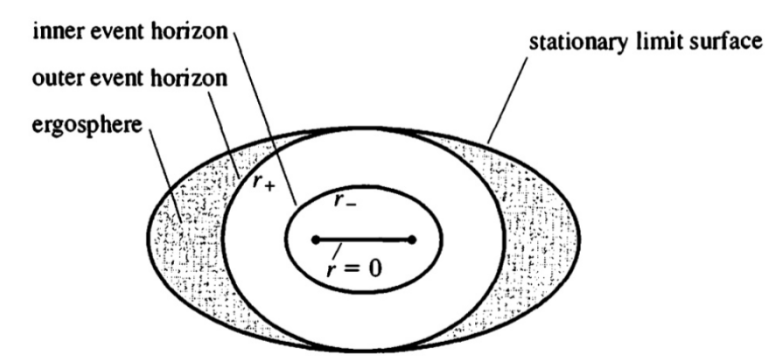
\includegraphics[scale=0.5]{img/imgRG6.16.PNG}
        \caption{Agujero negro de Kerr horizontes y ergosfera.}
    \end{figure}
\end{enumerate}

\section{Agujeros negros reales}

\textcolor{blue}{Estelares:} Son generados por el colapso gravitacional de una estrella con $M\geq 4 M_{\odot}$.
\begin{figure}[h]
    \centering
    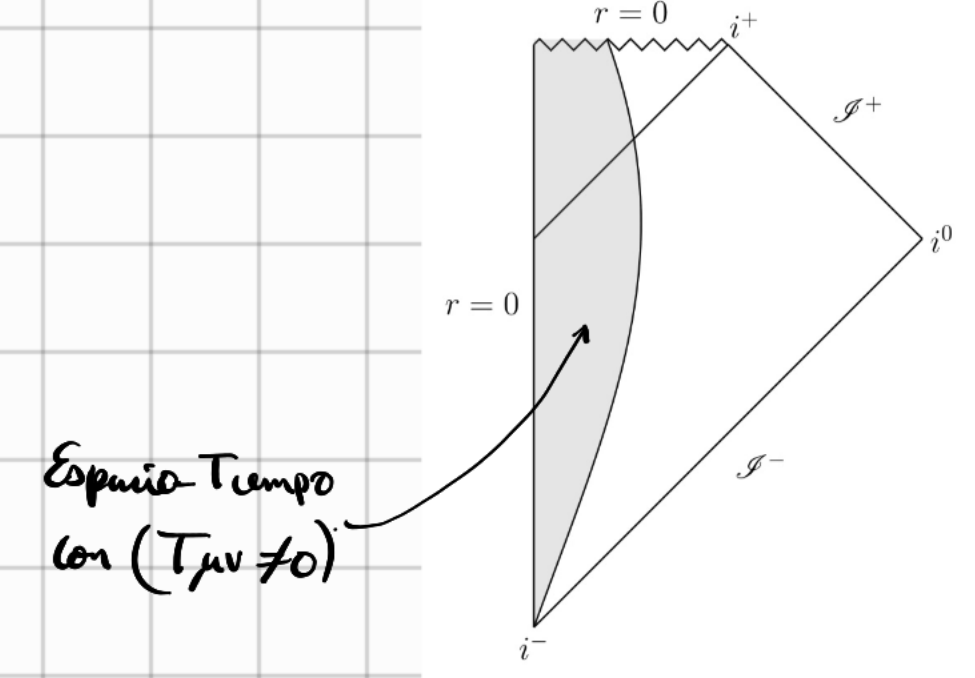
\includegraphics[scale=0.45]{img/imgRG6.17.PNG}
    \caption{Diagrama de Penrose para el colapso gravitacional de una estrella.}
\end{figure}

Nótese que la métrica adentro de la estrella corresponde a una solución diferente a la solución a las ecuaciones de Einstein en el vacío y que el colapso puede no ser homogéneo.
\begin{figure}[h]
    \centering
    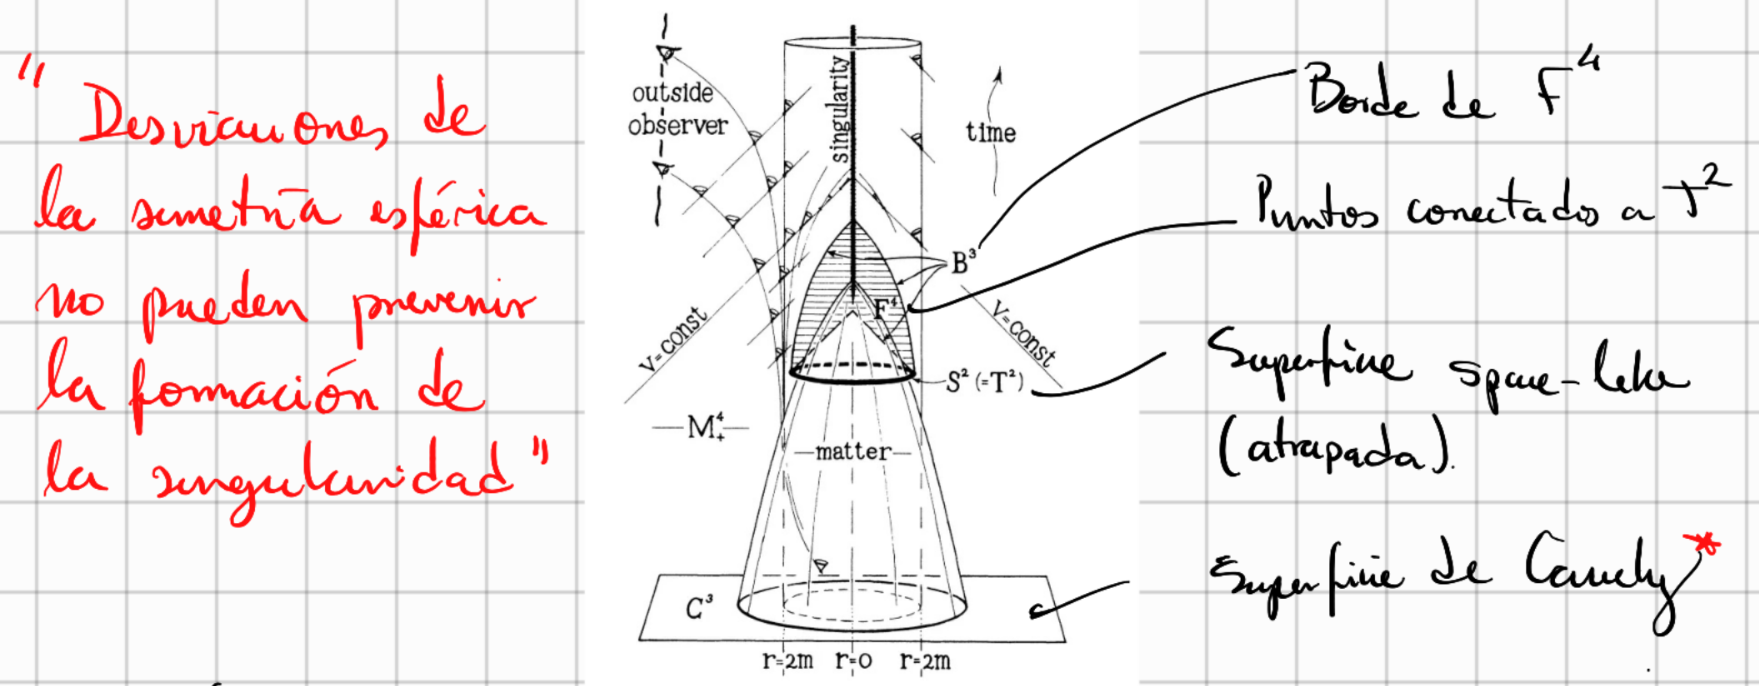
\includegraphics[scale=0.35]{img/imgRG6.18.PNG}
    \caption{Colapso gravitacional con simetría esférica.}
\end{figure}

En el gráfico anterior se describe el colapso de la materia y la formación de la singularidad.

En el colapso gravitacional con simetría esférica se asume:
\begin{enumerate}
    \item $M^4_+$: Es null-completa no singular.
    \item Las geodésicas en $M^4_+$ se pueden extender hacia el futuro usando un parámetro afín $\lambda \rightarrow + \infty$.
    \item Toda geodésica time-like nace con una superficie de Cauchy $C_3$.\footnote{Superficie de Cauchy: Es una submanifold con $t=constante$. Es usada para dar condiciones iniciales a las ecuaciones de Einstein.}
    \item Se cumple la condición $G_{\mu\nu}t^{\mu}t^{\nu}\geq 0$ para $t^{\mu}$ tipo tiempo \textcolor{red}{(condición de Energía no negativa).}
    \item Existe una superficie causalmente desconectada $T^2$.
\end{enumerate}

La inconsistencia de estas condiciones y la necesidad de una singularidad fue demostrada por Roger Penrose en 1965 al mostrar que $C_3$ debe ser una superficie de Cauchy \textcolor{red}{no compacta}.

\textcolor{blue}{Límite de Chandrasekhar:} En evolución estelar una estrella con masa suficientemente grande colapsará a una estrella de neutrones, sí la presión gravitacional supera la presión de degeneración de los electrones el límite para la formación de estos objetos es:
\begin{equation}
    M \approx 1.4M_{\odot}
\end{equation}

\section{Teoremas para agujeros negros}

En esta sección revisaremos algunos teoremas y condiciones involucrando agujeros negros:

\subsection{Condiciones de energía para un espacio-tiempo}
\begin{equation}
    T^{\mu\nu}=(\rho+p)u^{\mu}u^{\nu}+pg^{\mu\nu}
\end{equation}

\textbf{Condición de energía débil:} $T_{\mu\nu}t^{\mu}t^{\nu}\geq 0$ para cualquier vector time-like $t^{\mu}$. \textcolor{blue}{fluido perfecto $\rho\geq 0$ y $\rho+p\geq 0$}

\textbf{Condición de energía nula:} $T_{\mu\nu}t^{\mu}t^{\nu}\geq 0$ para cualquier vector nulo $t_{\mu}t^{\nu}=0$. \textcolor{blue}{fluido perfecto: $\rho+p\geq 0$.}

\textbf{Condición de energía fuerte:} $\displaystyle \left(T_{\mu\nu}-\dfrac{1}{2}g_{\mu\nu}T^{\alpha}_{\alpha}\right)t^{\mu} t^{\nu} \geq 0$ para cualquier vector time-like $t^{\mu}$. \textcolor{blue}{fluido perfecto $\rho+p\geq 0$ y $\rho+3p\geq 0$.}

\textbf{Condición de energía nula dominante:} $T_{\mu\nu}t^{\mu}t^{\nu}\geq 0$, para vectores $t^{\mu}$ con $t^{\mu}t_{\mu}=0$, además $T_{\mu\nu}t^{\nu}$ no puede ser un vector tipo space-like esta condición permite escribir $p=-\rho$.

\textbf{Condición de energía dominante:} $T_{\mu\nu}t^{\mu}t^{\nu}\geq 0$ con $t^{\mu}$ como un vector tipo time-like y además $T_{\mu\nu}t^{\nu}$ es un vector que no puede ser tipo space-like de esta definición se puede extraer $\rho \geq |p|$ en un fluido perfecto.

\subsection{Teorema de la singularidad de Penrose}

\teorema{} Sea $(\mathcal{M}, g)$ una manifold globalmente hiperbólica con una superficie de Cauchy no compacta. Asumiendo las ecuaciones de Einstein y la condición de energía nula y que $\mathcal{M}$ contiene una superficie causalmente desconectada $T$ sea $\theta_0<0$ el valor máximo de $\theta$ sobre $T$ en dos conjuntos de geodésicas nulas ortogonales a $T$. Luego, al menos una de esas geodésicas no es extendible para $\lambda \rightarrow + \infty$ con parámetro afín $\lambda \leq 2/\theta_0$.

\subsection{Teorema de no pelo}

\teorema{} Soluciones estacionarias y asintóticamente planas que son singulares fuera del horizonte de eventos están completamente caracterizados por la masa, carga eléctrica, carga magnética y el momento angular.

\subsection{Teorema de la singularidad}

\teorema{} Sea $\mathcal{M}$ una manifold con métrica genérica $g_{\mu\nu}$ que satisface las ecuaciones de Einstein. Sí existe alguna superficie causalmente desconectada en $\mathcal{M}$, debe entonces ser una curva cerrada tipo time-like o una singularidad.

\subsection{Teorema de la censura cósmica}

\teorema{} Singularidades desnudas no pueden formarse en colapso gravitacional de un espacio-tiempo genérico asintóticamente plano que obedezca la condición de energía dominante.

\subsection{Teorema del área de Hawking}

\teorema{} Asumiendo la condición de energía débil y el principio de censura cósmica, el área de un horizonte de eventos futuro en un espacio-tiempo asintóticamente plano no decrece.

\section{Procesos en agujeros negros}

\subsection{Horizonte de Killing}

Se define como la superficie $\Sigma$ donde $K^{\mu} K_{\mu}=0$. Un horizonte se puede relacionar con el horizonte de Killing sí:
\begin{enumerate}
    \item El espacio-tiempo es asintóticamente plano y estacionario el horizonte de eventos es también eun horizonte de Killing (es decir métrica de Schwarzschild).
    \item Sí e espacio-tiempo es estático $\xi^{\mu}$ será el vector de Killing $\xi^{\mu}=(\partial_t)^{\mu}$ representando las traslaciones temporales en el infinito.
    \item Sí el espacio-tiempo es estacionario pero no estático, el vector de Killing será una combinación lineal entre $(\partial_t)^{\mu}$ y $(\partial_{\phi})^{\mu}$.
    \begin{equation}
        \xi^{\mu}=(\partial_t)^{\mu}+\Omega_H(\partial_{\phi})^{\mu} \ \text{con} \ \Omega_H=cte
    \end{equation}
\end{enumerate}

\subsection{Proceso de Penrose}

Para un agujero negro de Kerr podemos calcular la energía y el momento angular de una partícula en una geodésica
\begin{align}
    E&=-(\partial_t)_{\mu}p^{\mu}=m\left(1-\dfrac{2GM}{p^2}\right)\dv{t}{\tau}+\dfrac{2mGMar}{\rho^2}\sin^2 \theta \dv{\phi}{\tau} \\
    L&=-(\partial_{\phi})_{\mu} p^{\mu}=-\dfrac{2mGMar}{\rho^2}\sin^2 \theta \dv{t}{\tau}+\dfrac{m(r^2+a^2)^2-m\Delta a^2\sin^2 \theta}{p^2}\sin^2\theta \dv{\phi}{\tau}
\end{align}
donde $E$ y $L$ son la energía y el momento angular por unidad de masa. Nótese que la definición de $E$ es compatible con la condición de energía positiva con el signo previamente escogido.

Dado que, el vector de Killing es tipo space-like en la métrica de Kerr cuando estamos dentro de la ergosfera del agujero negro. Como las partículas deben acelerar para salir de esta región.

Un decaimiento de una partícula en esta región llevaria a un aumento en la energía de uno de los subproductos del decaimiento así 
\begin{align}
    p^{\mu}&=p^{\mu}_1+p^{\mu}_2 \\
    E&=E_1+E_2
\end{align}
\begin{figure}[h]
    \centering
    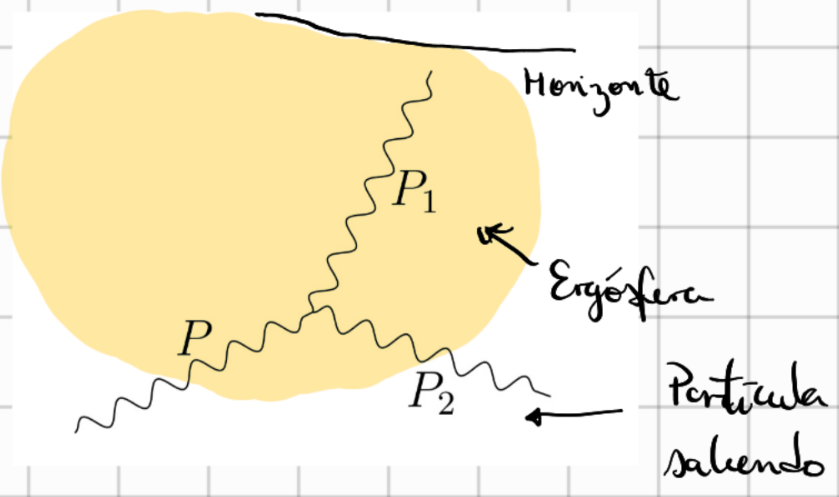
\includegraphics[scale=0.5]{img/imgRG6.19.PNG}
\end{figure}

Sí la partículas 1 permanece en la ergosfera $E_1$ puede ser negativa y $E_2$
\begin{equation}
    E_2=E+|E_1|>E
\end{equation}

Sí la partícula 1 cae en el agujero negro y la partícula 2 escapa a infinito resultando en una perdida de energía para el agujero negro. La extracción de energía de este tipo se llama \textcolor{red}{Proceso de Penrose.}

Se puede mostrar que el agujero negro resultante tendrá un momento angular ligeramente diferente:
\begin{equation}
    \delta J < \dfrac{\delta M}{\Omega_H}=\dfrac{2M(M^2+\sqrt{M^4-J^2})}{J}\delta M \ \text{y} \ \Omega_M=\left(\dv{\phi}{t}\right)(r_+)
\end{equation}

Existiendo un límite para la cantidad de masa que se puede extraer con este proceso
\begin{equation}
    M^2=M^2_{irr}+\dfrac{J^2}{4M^2_{irr}}\geq M^2_{irr}
\end{equation}

Donde $M_{irr}$, es la masa irreducible del agujero negro.
\begin{equation}
    M_{irr}=\sqrt{\dfrac{1}{2}\left(M^2+\sqrt{M^4-J^2}\right)}
\end{equation}

Se puede mostrar que usando la definición de area $A$
\begin{equation}
    A=\int \sqrt{|y|}\mathrm{d}t \mathrm{d}\phi
\end{equation}
donde $y$ es la métrica con: $\mathrm{d}t=0, \mathrm{d}r=0$ y $r=r_+$ y para la solución de Kerr:
\begin{equation}
    y_{ij}\mathrm{d}x^{i}\mathrm{d}x^{j}=(r^2_{+}+a^2\cos^2 \theta)\mathrm{d}t^2+\left[\dfrac{(r^2_{+} +a^2)^2\sin^2 \theta}{r^2_{+} +a^2\cos^2 \theta}\right]\mathrm{d}\phi^2
\end{equation}

El área en $r_+$ está dada por:
\begin{equation}
    A=4\pi(r^2_{+}+a^2)
\end{equation}
con $r_+$ como el horizonte externo, usando 
\begin{equation}
    M^2_{irr}=\dfrac{A}{16\pi G}
\end{equation}
y variando $\delta M_{irr}$ y $\delta A$ se puede obtener:
\begin{equation}
    \delta A=\dfrac{8\pi G a(\delta M-\Omega_H \delta J)}{\Omega_H\sqrt{G^2 M^2-a^2}}
\end{equation}

Donde introduciendo la cantidad $\kappa$ o gravedad superficial 
\begin{equation}
    \kappa=\dfrac{(G^2M^2-a^2)^{1/2}}{2GM(GM+\sqrt{G^2M^2-a^2})}
\end{equation}

Podemos escribir, donde $\delta A>0$ vemos que
\begin{equation}
    \delta M=\dfrac{\kappa}{8\pi G}\delta A+\Omega_M \delta J
\end{equation}
ecuación que puede ser mapeada a la 1ra ley de la termodinámica usando 
\begin{equation}
    \mathrm{d}E=T\mathrm{d}S-p\mathrm{d}V
\end{equation}
con $E\rightarrow M, S \rightarrow A/4\pi G$ y $T\rightarrow \kappa/2\pi$.

Donde, para $T=\kappa/2\pi$ podemos interpretar $A/4\pi G$ como la entropia del agujero negro(Hawking).

También es posible escribir la segunda ley de la termodinámica de forma generalizada(Bekenstein):
\begin{equation}
    \delta\left(S+\dfrac{A}{4G}\right)\geq 0
\end{equation}

\subsection{La ecuación de Landau-Raychaudhuri}
Determina la evolución de la expansión $\theta$ de una congruencia de tipo time-like. Es decir, mide el cambio fraccional de un volumen de materia medido por un observador comovil. Para un vector tipo time-like $x^{\mu}$, la congruencia de geodésicas en el punto $p$ evoluciona como:
\begin{equation}
    \dv{\theta}{\lambda}=-\dfrac{\theta^2}{2}-\hat{\sigma}^{\mu\nu}\hat{\sigma}_{\mu\nu}+w^{\mu\nu}w_{\mu\nu}-R_{\mu\nu}u^{\mu}u^{\nu}
\end{equation}
donde $\sigma_{\mu\nu}$ y $w^{\mu\nu}$ son el cizallamiento(shear) y la vorticidad(vorticity) respectivamente, definidos como:
\begin{equation}
    \sigma=\hat{B}^{\mu}_{\mu},\quad \hat{\sigma}_{\mu\nu}=\hat{B}_{(\mu\nu)}-\dfrac{1}{2}p_{\mu\nu}\sigma,\quad w_{\mu\nu}=\hat{B}_{(\mu\nu)}
\end{equation}

Nótese que $p_{\mu\nu}$ es un proyector de la forma:
\begin{equation}
    p^{\nu}_{\mu}=\delta^{\nu}_{\mu}+N^{\nu}u_{\mu}+u^{\nu}N_{\mu}
\end{equation}
donde $B_{\mu\nu}=\nabla_{\mu}u_{\nu}$ y $u_{\mu}$ es un vector tangente $u^2=\pm 1$. Esta definición se usa para demostrar el teorema de Penrose para una hipersuperficie nula con $\displaystyle \dv{\theta}{\lambda}\leq -\dfrac{1}{2}\theta^2$.

\section*{Problemas 4}

\begin{enumerate}
    \item \textbf{Resolviendo las Ecuaciones de Einstein con Constante Cosmológica}
    Considere las ecuaciones de Einstein en el vacío, pero con una constante cosmológica positiva $\Lambda >0$
    \begin{equation}
        G_{\mu\nu}+\Lambda g_{\mu\nu}=0.
        \label{ec6.106}
    \end{equation}
    \begin{enumerate}[label=(\alph*)]
        \item Muestre que las soluciones a la Eq. \eqref{ec6.106} también satisfacen $R_{\mu\nu}=\Lambda g_{\mu\nu}$.
        \item Suponga un ansatz para una métrica estática, esféricamente simétrica, y que en coordenadas $(t, r, \theta, \phi)$ se reducen a las coordenadas de Schwarzschild en el límite $\Lambda =0$, de la forma
        \begin{equation}
            g_{\mu\nu}\mathrm{d}x^{\mu}\mathrm{d}x^{\nu}=-A(r)\mathrm{d}t^2+B(r)\mathrm{d}r^2+r^2\left[\mathrm{d}\theta^2+\sin^2(\theta)\mathrm{d}\phi^2\right],
        \end{equation}
        donde $A(r)$ y $B(r)$ son funciones desconocidas que solo dependen de $r$. Con este ansatz, calcule las componentes del tensor de Ricci y determine las ecuaciones diferenciales que se deben resolver para $A(r)$ y $B(r)$.
        \item Muestre que una condición que deben satisfacer ambas funciones es: $A(r)B(r)=1.$
        \item Integrando las ecuaciones diferenciales que aparecen en el resto de las componentes del tensor de Ricci, encuentre la solución general para ambas funciones. Determine las constantes de integración comparando con el límite $\Lambda =0$, y escriba la forma final de la métrica.
    \end{enumerate}
    \item \textbf{Preámbulo: Agujeros Negros}
    Hacer un resumen detallado de cada capítulo del 4 al 9 del libro ``\textit{Black Holes: The Key to Understanding the Universe}'' de Brian Cox y Jeff Forshaw. (Mínimo 900 palabras por capítulo, usar únicamente \LaTeX para esto).
    \item \textbf{Diagrama de Carter-Penrose}
    Consideremos el espacio de Minkowski de cuatro dimensiones en coordenadas polares,
    \begin{equation}
        \mathrm{d}s^2=-\mathrm{d}t^2+\mathrm{d}r^2+r^2\mathrm{d}\Omega^2_2,\ \mathrm{d}\Omega^2_2=\mathrm{d}\theta^2+\sin^2 \theta \mathrm{d}\phi^2.
    \end{equation}
    \begin{enumerate}[label=(\alph*)]
        \item Demuestra que el cambio de coordenadas 
        \begin{equation}
            (r+t)=\tan\left(\dfrac{R+T}{2}\right) \quad \text{y} \quad (r-t)=\tan\left(\dfrac{R-T}{2}\right)
        \end{equation}
        da como resultado la métrica,
        \begin{equation}
            \mathrm{d}s^2=f(T, R)(-\mathrm{d}T^2+\mathrm{d}R^2+\sin^2(R)\mathrm{d}\Omega^2_2)
        \end{equation}
        y determina la función $f(T, R)$.
        \item Indica los rangos de coordenadas para el tiempo $T$ y la coordenada radial $R$ en los cuales el espacio de Minkowski está completamente cubierto una vez en las nuevas coordenadas.
        \item Dibuje el diagrama de Carter-Penrose e identifica $i^{\pm}, i^0, \mathcal{J}^{\pm}$. 
        \item Proporciona la parametrización de las siguientes geodésicas que pasan por el origen $R=0$:
        \begin{enumerate}
            \item Rayos de luz.
            \item Dos geodésicas distintas de tipo tiempo.
            \item Dos geodésicas distintas de tipo espacio. Dibuja las geodésicas cualitativamente en el diagrama de Penrose.
        \end{enumerate}
    \end{enumerate}
    \item \textbf{Resolviendo la singularidad de Schwarzschild}
    En la solución de Schwarzschild una singularidad aparece al acercarse al radio de Schwarzschild, siendo este un efecto de coordenadas, en este ejercicio encontraremos las coordenadas en las que esta singularidad desaparece.
    \begin{enumerate}[label=(\alph*)]
        \item Muestre que la métrica de Schwarzschild presenta una singularidad en $r=2GM$.
        \begin{equation}
            \mathrm{d}s^2=-\left(1-\dfrac{2GM}{r}\right)\mathrm{d}t^2+\left(1-\dfrac{2GM}{r}\right)^{-1}\mathrm{d}r^2+r^2\mathrm{d}\Omega^2.
        \end{equation}
        \item Muestra que se pueden usar las llamadas ``coordenadas de tortuga'' definidas como:
        \begin{equation}
            r^*=r+2GM\ln\left(\dfrac{r}{2GM}-1\right)
        \end{equation}
        para llevar la métrica de Schwarzschild a la forma:
        \begin{equation}
            \mathrm{d}s^2=\left(1-\dfrac{2GM}{r}\right)(-\mathrm{d}t^2+\mathrm{d}r^*{}^2)+r^2\mathrm{d}\Omega^2
        \end{equation}
        \item Luego muestre que las coordenadas de Eddington-Finkelstein, combinando $r^*$ y $t$, escritas como:
        \begin{equation}
            \tilde{u}=t+r^*, \quad \tilde{v}=t-r^*.
        \end{equation}
        estas coordenadas reescriben la métrica como:
        \begin{equation}
            \mathrm{d}s^2=\dfrac{1}{2}\left(1-\dfrac{2GM}{r}\right)(\mathrm{d}\tilde{u}\mathrm{d}\tilde{v}+\mathrm{d}\tilde{v}\mathrm{d}\tilde{u})+r^2\mathrm{d}\Omega^2
        \end{equation}
        \item Finalmente para regularizar la métrica, introducimos las coordenadas de Kruskal-Szekeres donde:
        \begin{align}
            u'&=e^{\tilde{u}/4GM},\\
            v'&=e^{-\tilde{v}/4GM}.
        \end{align}
        \vspace{-0.7cm}
        \begin{align}
            u'&=\left(\dfrac{r}{2GM}-1\right)^{1/2}e^{(r+t)/4GM},\\
            v'&=\left(\dfrac{r}{2GM}-1\right)^{1/2}e^{(r-t)/4GM}.
        \end{align}
        \item Muestre que en términos de estas últimas nuevas coordenadas, la métrica se convierte en:
        \begin{equation}
            \mathrm{d}s^2=-\dfrac{16G^3 M^3}{r}e^{-r/2GM}(\mathrm{d}u'\mathrm{d}v'+\mathrm{d}v'\mathrm{d}u')+r^2\mathrm{d}\Omega^2
        \end{equation}
    \end{enumerate}
    \item \textbf{Agujero Negro Reissner-Nordström}
    En la presencia de un campo electromagnético, una partícula de carga $e$ y masa $m$ obedece la versión relativista de la segunda ley de Newton, $f^{\mu}=ma^{\mu}$, o explícitamente:
    \begin{equation}
        \dv{^2 x^{\mu}}{\tau^2}+\Gamma^{\mu}_{\rho\sigma}\dv{x^{\rho}}{\tau}\dv{x^{\sigma}}{\tau}=\dfrac{e}{m}F^{\mu}_{\nu}\dv{x^{\nu}}{\tau}
    \end{equation}
    donde $F_{\mu\nu}$ son las componentes del tensor de Maxwell, que se pueden escribir en términos del 4-potencial como $F_{\mu\nu}=\partial_{\mu}A_{\nu}-\partial_{\nu}A_{\mu}$. Imagine que dicha partícula se mueve a través de un espacio-tiempo de Reissner-Nordström, descrito por la métrica 
    \begin{equation}
        g_{\mu\nu}\mathrm{d}x^{\mu}\mathrm{d}x^{\nu}=-\left(1-\dfrac{r_s}{r}+\dfrac{r^2_Q}{r^2}\right)\mathrm{d}t^2+\left(1-\dfrac{r_s}{r}+\dfrac{r^2_Q}{r^2}\right)^{-1}\mathrm{d}r^2+r^2\left[\mathrm{d}\theta^2+\sin^2(\theta)\mathrm{d}\phi^2\right],
    \end{equation}
    donde $r_s=2GM$ y $r^2_Q=Q^2G$. Considere unidades en donde $c=4\pi \epsilon_0=1$.
    \begin{enumerate}[label=(\alph*)]
        \item Muestre que la energía de la partícula, dada por 
        \begin{equation}
            E=m\left(1-\dfrac{2GM}{r}+\dfrac{Q^2 G}{r^2}\right)\dv{t}{\tau}+\dfrac{eQ}{r},
        \end{equation}
        es una cantidad conservada.
        \item ¿Podrá un proceso tipo Penrose realizar trabajo para un agujero negro cargado? ¿Cuál es el cambio en la masa del agujero negro, $\delta M$, para el proceso física máximo?
    \end{enumerate}
    \item \textbf{Agujero Negro BTZ}
    \begin{enumerate}[label=(\alph*)]
        \item Considere la siguiente métrica de un espacio-tiempo tridimensional $(2+1)$:
        \begin{equation}
            g_{\mu\nu}\mathrm{d}x^{\mu}\mathrm{d}x^{\nu}=-f(r)\mathrm{d}t^2+\dfrac{1}{f(r)}\mathrm{d}r^2+r^2\left(\mathrm{d}\phi-\dfrac{r_{+}r_{-}}{\ell r^2}\mathrm{d}t\right)^2, \ f(r)=\dfrac{(r^2-r^2_+)(r^2-r^2_-)}{\ell^2 r^2}
        \end{equation}
        \begin{enumerate}[label=(\alph*)]
            \item Para una partícula de prueba en esta geometría, escriba explícitamente las dos cantidades conservadas asociadas a las simetrías que tiene esa métrica.
            \item Muestre que si $r_+ r_- \neq 0$, entonces el agujero negro está rotando.
            \item Suponga que existe un observador que se mantiene a una distancia coordenada radial fija $r=R$. Muestre que es imposible debajo de cierto radio mantenerse a un ángulo fijo, es decir, los observadores están forzados a rotar juntos con el agujero negro. 
            \item Considere que dos observadores se mantengan a una distancia radial y ángulos fijos. Uno envía una señal electromagnética al otro. Con esta información, calcule el redshift gravitacional.
        \end{enumerate}
    \end{enumerate}
\end{enumerate}
\end{document}